\subsection{Nabavka}

\begin{figure}[ht]
\centering
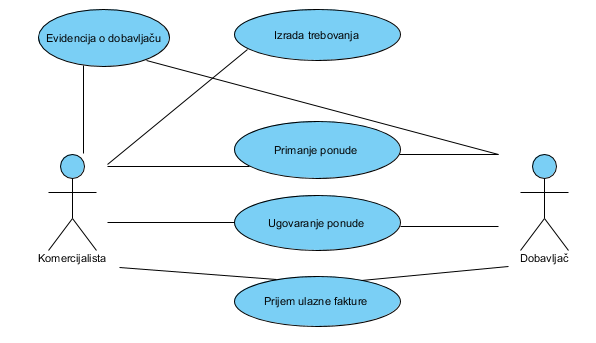
\includegraphics[width=120mm]{slike/useCaseNabavka.png}
\caption{Dijagram slučajeva upotrebe vezanih za nabavku}
\end{figure}

\clearpage

\subsubsection{Evidencija dobavljaca}

\textbf{Opis:}

Evidentiranje dobavljača kao pravnog lica i kontakt osobe iz te firme.
\newline
\textbf{Akteri:}

Dobavljač- daje potrebne informacije

Komercijalista- traži od dobavljača potrebne informacije
\newline
\textbf{Preduslov:}

Ostvaren je kontakt sa dobavljačem ili se planira saradnja
\newline
\textbf{Postuslov:}

Uspšno uneti podaci u bazu
\newline
\textbf{Glavni tok:}

1. Komercijalista ulazi u deo programa koji se bavi evidencijom.

2. Prikazuje se tabela sa svim unešenim dobavljačima. 

Zatim slede koraci u zavisnosti od potrebnog.

\textit{Čitanje}

1. Klikom na konkretnog dobavljača prikazuju mu se detaljnije informacije o dobavljaču tj. firmi o kojima imamo podatke.

\textit{Dodavanje}

1. Opcija "Dodaj novog dobavljača" otvara formu za unos, unosi podatke o firmi iz APR(Agencija za privredne registre) koji su dostupni sa interneta.

\textit{Ažuriranje}

1. Opcija ”Izmene” postoji pored svakog postojećeg dobavljača. Pomoću koje menjamo postojeće podatke.

2. Klikom opcije ”Izmena” pored postojećih dobavljača menjamo podatke o njima.

\textit{Brisanje}

1. Opcija ”Obriši” postoji pored svakog postojećeg dobavljača pomoću koje brišemo postojeće podatke.

2. Klikom opcije ”Obriši” pored postojećih dobavljača brišemo podatke o njima.

\clearpage

\subsubsection{Izrada trebovanja}

\textbf{Opis:}

Evidentiranje robe koje više nema na stanju i robe koje će nam biti potrebna za prodaju. Izrada trebovanja za nabavljanje te robe.
\newline
\textbf{Akteri:}

Komercijalista - Proverava šta od robe više nema na stanju i odlučuje se za novu robu koju naručuje.

Menadžer - može uticati na izradu trebovanja nekom svojom politikom ili uvesti novu robu u poslovanje firme 
\newline
\textbf{Preduslov:}

Manjak robe na stanju.
\newline
\textbf{Postuslov:}

Naračena roba za dalje poslovanje.
\newline
\textbf{Glavni tok:}

1. Komercijalista primećuje da je neke robe nestalo sa stanja ili zeli da naruči novu robu.

2. Komercijalista vrši popis robe koja je nestala i odlučuje se za željenu količinu.
Ulazi u deo programa za nabavku, kreira novo trebovanje.

3. Komercijalista kontaktira dobavljača i naručuje robu.
\newline
\textbf{Alternativni tok:}
2.1 Menadžer eventualno daje svoje predloge za trebovanje.
\newline
\textbf{Napomena:}
Ne treba doći u situaciju da nema robe na stanju u magacinu. Već konstantno naručivati potrebne količine. Uglavnom, porudžbina se ne pravi za svako posebno trebovanje, već za više njih.

\subsubsection{Primanje ponude}

\textbf{Opis:}

Dobavljač nudi robu, koju komercijalista odlučuje da primi ili odbije.
\newline
\textbf{Akteri:}

Dobavljač- nudi novu robu

Komercijalista- razmatra ponudu
\newline
\textbf{Preduslov:}

Dobavljač je registrovan u bazi dobavljača.
\newline
\textbf{Postuslov:}

Ponuda seštena u bazu.
\newline
\textbf{Glavni tok:}

1. Dobavljač kontaktira komercijalistu i šalje mu ponudu poručenih lekova.

2. Komercijalista u delu programa za nabavku, pod ponudama skladišti ponude.

3. Komercijalista razmatra ponudu.
\newline
\textbf{Izlazni dokument:}

Porudžbina sačuvana u bazi.


\subsubsection{Ugovaranje ponude}

\textbf{Opis:}

Ugovaranje ponude sa dobavljačem, u cilju ostvarivanje prodaje na obostrano zadovoljstvo.
\newline
\textbf{Akteri:}

Dobavljač- predstavlja ponudu i koriguje je u skladu sa zahtevima komercijaliste

Komercijalista- prihvata ili odbija ponudu dobavljaca

\textbf{Preduslov:}

Ponuda uneta i postoji u bazi podataka.
\newline
\textbf{Postuslov:}

Obe strane zadovoljne poslom, kupovina ce se izvršiti.
\newline
\textbf{Glavni tok:}

1. Komercijalista se izjašnjava oko ponude.

2. Komercijalista pristaje na ponudu.

\textbf{Alternativni tok:}

1.1. Komercijalista nije u potpunosti zadovoljan ponudom

1.2. Dobavljač u dogovoru sa komercijalistom ažurira ponudu

1.3. Dobavljač pravi novu poboljšanu ponudu.

\textbf{Drugi alternativni tok:}

2. Kupcu ne odgovara ponuda.

3. Trenutna saradnja se završava.


\subsubsection{Prijem ulaznih faktura}

\textbf{Opis:}

Prihvatanje fakture od dobavljača.
\newline
\textbf{Akteri:}

Komercijalista- evidentira pristigle fakture

Dobavljač- Šalje fakutre
\newline
\textbf{Preduslov:}

Postoji narudžbina za koju se šalje faktura.
\newline
\textbf{Postuslov:}

Faktura prihvaćena i evidentirana.
\newline
\textbf{Glavni tok:}

1. Dobavljač uz porudžbinu šalje i fakturu

2. Komercijalista prihvata fakuturu

3. Komercijalista ulazi u deo programa za nabavku, pod fakturama, kreira novu.
\newline
\textbf{Alternativni tok:}

1.1 Dobavljač zaboravio da pošalje fakturu.

1.2 Komercijalista ga kontaktira i naknadno trazi da se pošalje faktura.
\newline
\clearpage